\subsection{Sum and Product}\label{ssec:sum_prod}

\begin{figure*}[t]
    \centering
    \begin{subfigure}[b]{0.475\textwidth}
        \centering
        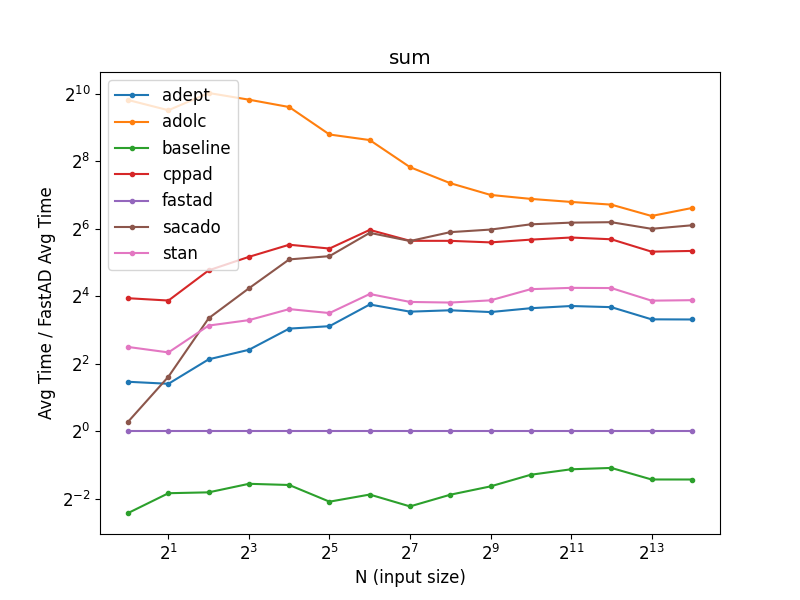
\includegraphics[width=\textwidth]{figs/sum_fig.png}
        \caption{Sum}\label{fig:sum}
    \end{subfigure}
    \hfill
    \begin{subfigure}[b]{0.475\textwidth}
        \centering
        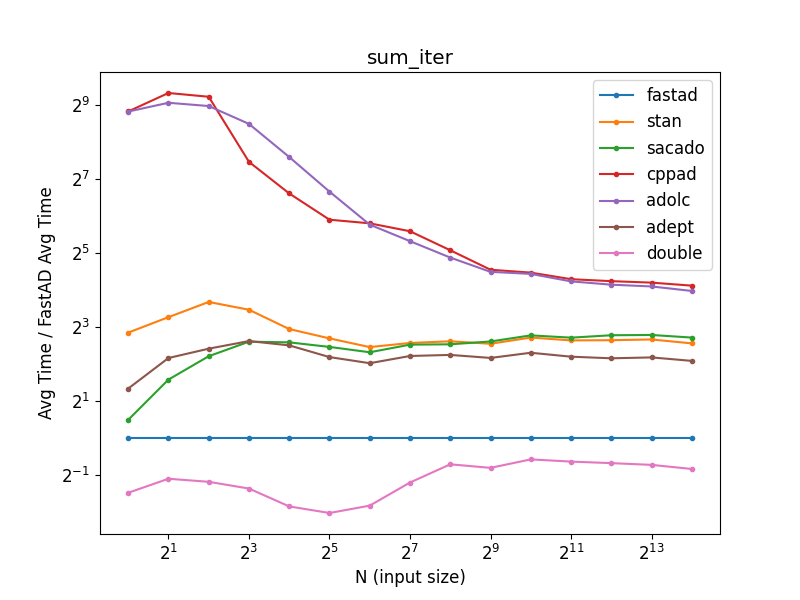
\includegraphics[width=\textwidth]{figs/sum_iter_fig.png}
        \caption{Sum (naive, for-loop-based)}\label{fig:sum_iter}
    \end{subfigure}
    \vskip\baselineskip%
    \begin{subfigure}[b]{0.475\textwidth}
        \centering
        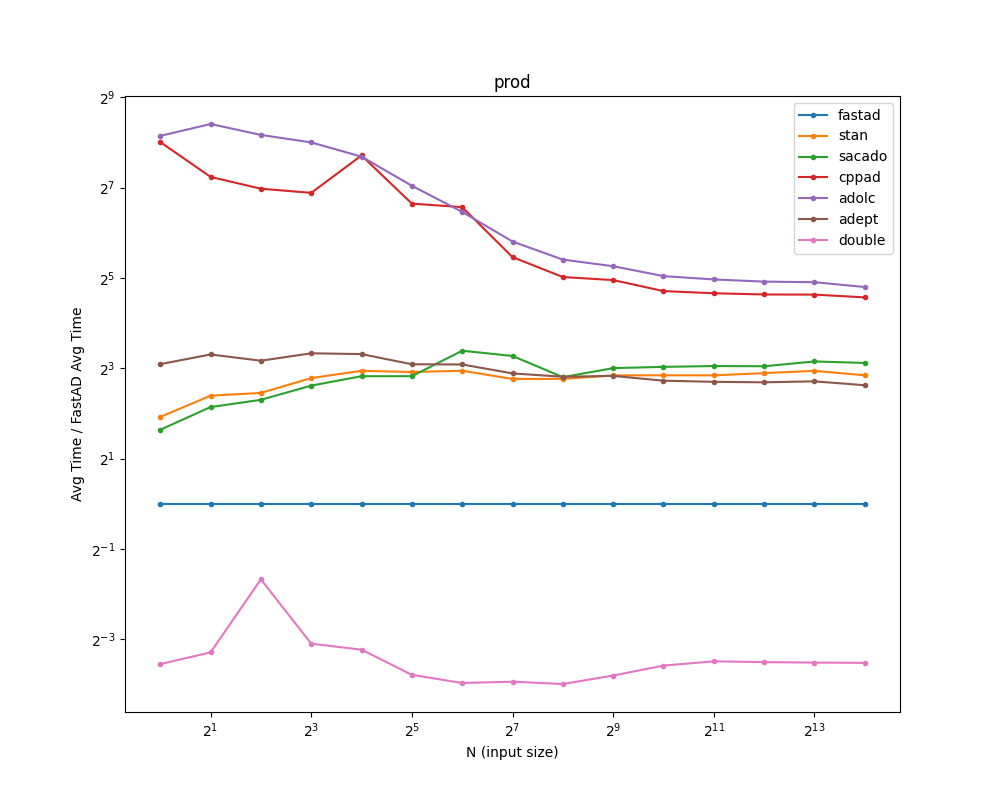
\includegraphics[width=\textwidth]{figs/prod_fig.png}
        \caption{Product}\label{fig:prod}
    \end{subfigure}
    \hfill
    \begin{subfigure}[b]{0.475\textwidth}
        \centering
        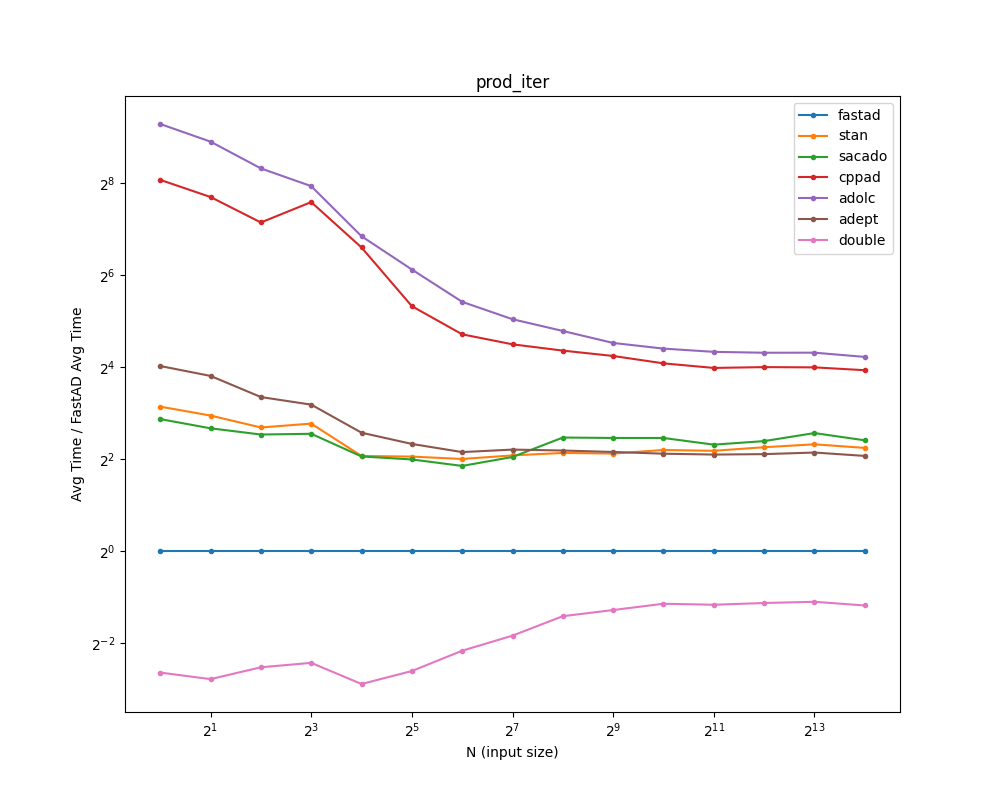
\includegraphics[width=\textwidth]{figs/prod_iter_fig.png}
        \caption{Product (naive, for-loop-based)}\label{fig:prod_iter}
    \end{subfigure}
    \caption{%
        Sum and product benchmarks of other libraries against FastAD 
        plotted relative to FastAD average time.
        Fig.~\ref{fig:sum},\ref{fig:prod} use built-in functions whenever available.
        Fig.~\ref{fig:sum_iter},\ref{fig:prod_iter} use the naive iterative-based code for all libraries.
    }\label{fig:sum_prod}
\end{figure*}

The summation function is defined as $f_s:\R^n \to \R$ where~$f_s(x) = \sum\limits_{i=1}^n x_i$,
and the product function is defined as $f_p:\R^n \to \R$ where~$f_p(x) = \prod\limits_{i=1}^n x_i$.
The only libraries supporting a built-in function for summation are Adept, FastAD, and Stan;
those that support product are Adept and FastAD.
As another test, we forced all libraries to use a manually-written for-loop-based summation and product.
Fig.\ref{fig:sum_prod} shows the benchmark results.

In all four cases, it is clear that FastAD outperforms all libraries for all values of $N$
by a significant factor.
For \code{sum}, 
the next three fastest libraries, asymptotically, are Adept, Stan, and Sacado, respectively.
The trend stabilizes starting from $N=2^6=64$ where Adept is about $ 12$ times slower than
FastAD, Stan about $ 18$ times, and Sacado about $ 74$ times.
The naive, for-loop-based benchmark shown in Fig.\ref{fig:sum_iter} exhibits a similar pattern,
although the performance difference with FastAD is less extreme:
Adept is about $ 4$ times slower, 
Stan about $ 6$ times,
and Sacado about $ 6.5$ times.
Nonetheless, this is still a very notable difference.

For the \code{prod} and \code{prod\_iter} cases, 
Fig.\ref{fig:prod},\ref{fig:prod_iter} again show
a similar trend as \code{sum} and \code{sum\_iter}.
Overall, the comparison with FastAD is less extreme.
For \code{prod}, Adept is about $ 5.6$ times slower than FastAD,
Stan about $ 7.3$ times slower,
and Sacado about $ 16.4$ times slower.
For \code{prod\_iter}, Adept is about $2.9$ times slower,
Stan about $4$ times slower,
and Sacado about $4.6$ times slower.
